\documentclass{article}

%\usepackage{corl_2026} % Use this for the initial submission.
\usepackage[final]{corl_2026} % Uncomment for the camera-ready ``final'' version.
%\usepackage[preprint]{corl_2026} % Uncomment for pre-prints (e.g., arxiv); This is like ``final'', but will remove the CORL footnote.
\begin{document}


%===============================================================================
We present two reinforcement learning agents for the Soccer Twos environment. Agent 1 uses Proximal Policy Optimization (PPO) with curriculum learning, self-play style opponents, and dense reward shaping to address the sparse goal-scoring reward. Agent 2 uses Deep Q-Networks (DQN) with a custom observation transformation wrapper that extracts spatially-relevant features, enabling faster convergence and more robust action-value learning.


\subsection*{Method Description}

\subsection*{Agent 1: PPO with Curriculum Learning and Reward Shaping}

Agent 1 was trained using Proximal Policy Optimization (PPO) implemented with Ray RLlib using the PyTorch backend. PPO is an on-policy actor-critic reinforcement learning algorithm. The policy network, or actor, outputs a distribution over actions, while the value function, or critic, estimates the expected return from the current state. During training, PPO collects rollouts using the current policy, estimates advantages from the difference between observed returns and value predictions, and then updates the policy to increase the probability of actions with positive advantage.

The main stability mechanism in PPO is the clipped surrogate objective. This discourages destructive updates that would change the policy too quickly. In Soccer Twos, this is useful because the action space is discrete and multi-branch, the reward is sparse, and poor updates can easily destroy useful movement or ball-control behaviors.

The architecture used for Agent 1 was a feed-forward neural network with two hidden layers of 512 units. The policy and value function shared these hidden layers (\texttt{vf\_share\_layers=True}), which reduces the number of parameters and lets both heads learn from the same representation of player and ball state.

\subsubsection*{Final Training Hyperparameters}

\begin{center}
\begin{tabular}{|l|l|}
\hline
\textbf{Hyperparameter} & \textbf{Agent 1 Value} \\
\hline
Algorithm & PPO \\
\hline
Library & Ray RLlib 1.4.0 with PyTorch \\
\hline
Learning rate & RLlib PPO default, not manually overridden \\
\hline
Training batch size & RLlib PPO default, not manually overridden \\
\hline
Replay/buffer size & Not applicable; PPO is on-policy and does not use a replay buffer \\
\hline
Environment variation & \texttt{EnvType.team\_vs\_policy} \\
\hline
Multi-agent wrapper & Disabled during training (\texttt{multiagent=False}) \\
\hline
Number of rollout workers & 16 \\
\hline
Environments per worker & 1 \\
\hline
GPU count & 0 \\
\hline
Rollout fragment length & 3000 \\
\hline
Batch mode & Complete episodes \\
\hline
Network hidden layers & $[512, 512]$ \\
\hline
Value-function layer sharing & Enabled \\
\hline
Reward shaping & Enabled \\
\hline
Progress shaping weight & 1.0 \\
\hline
Distance shaping weight & 0.35 \\
\hline
Alignment shaping weight & 0.08 \\
\hline
Progress scale & 20.0 \\
\hline
Distance scale & 12.0 \\
\hline
Maximum shaping reward per step & 0.05 \\
\hline
Checkpoint selected & \texttt{checkpoint-1794} \\
\hline
\end{tabular}
\end{center}

Parameters not explicitly overridden in the training configuration, such as PPO's learning rate, minibatch size, discount factor, clipping coefficient, and number of SGD passes, used the default values from Ray RLlib PPO.

\subsubsection{Specific Modification}

The main modification for Agent 1 was reward shaping. The original Soccer Twos environment gives sparse rewards that are mainly tied to scoring or conceding goals. This makes exploration difficult because many episodes provide little feedback about whether the agent is moving in a useful direction. To make the learning signal denser, we added a \texttt{PotentialRewardShapingWrapper} in \texttt{utils.py}. This wrapper keeps the original environment reward and adds a bounded shaping term:
\[
R_{total} = R_{extrinsic} + R_{shaping}.
\]

The shaping reward is computed as the change in a potential function between consecutive states:
\[
R_{shaping} = \mathrm{clip}(\Phi(s_{t+1}) - \Phi(s_t), -c, c),
\]
where $c$ is the maximum absolute shaping reward per step. The potential function combines three task-relevant terms:
\[
\Phi(s) =
w_p \cdot \mathrm{ball\ progress}
+ w_d \cdot \mathrm{player\ ball\ distance}
+ w_a \cdot \mathrm{ball\ velocity\ alignment}.
\]

The progress term rewards moving the ball toward the opponent goal, the distance term rewards keeping the controlled player close to the ball, and the alignment term rewards ball velocity pointing toward the opponent goal. The final curriculum checkpoint used progress weight 1.0, distance weight 0.35, alignment weight 0.08, and maximum shaping magnitude 0.05.

Agent 1 also used curriculum learning. Early stages initialized the ball and players near easier scoring positions, while later stages expanded the initial-state ranges and introduced harder opponents. The curriculum advanced based on win rate, non-loss rate, and extrinsic return. This let the policy first learn basic approach and scoring behavior before being exposed to more realistic full-field situations.

\subsubsection{Hypothesis and Motivation}

The hypothesis behind reward shaping was that Soccer Twos is too sparse for efficient early PPO learning if the agent only receives useful feedback after goals. A random or weak policy rarely scores, so the policy gradient can have high variance and little information about intermediate behaviors such as approaching the ball, pushing it forward, or shooting toward the goal. By adding potential-based dense feedback, we expected the agent to discover useful soccer primitives faster while still preserving the sparse goal reward as the main objective.

The motivation for curriculum learning was similar. Starting directly from fully random full-field states can make the first successful scoring trajectories extremely rare. Easier initial states reduce the exploration burden and teach the policy behaviors that transfer to harder stages. As the curriculum expands the state distribution and opponent difficulty, the policy is forced to keep those useful behaviors while becoming more robust.

\subsection{Agent 2: DQN with Custom Observation Wrapper}

\subsubsection{Algorithm, Library, and Theoretical Background}

Agent 2 uses Deep Q-Networks (DQN) with Ray RLlib (PyTorch backend), an off-policy value-based algorithm that learns action-value functions by minimizing TD error. The implementation incorporates several advanced techniques: Double DQN (reduces overestimation bias), 3-step returns (reduces variance), dueling architecture (separates value and advantage learning), Prioritized Experience Replay (focuses on high-error transitions), and distributional RL with 51 atoms (learns return distributions). Actions are selected via $\epsilon$-greedy exploration with Noisy Nets for efficient exploration.

\subsubsection{Final Training Hyperparameters}

\begin{center}
\begin{tabular}{|l|l|}
\hline
\textbf{Hyperparameter} & \textbf{Agent 2 Value} \\
\hline
Algorithm & DQN \\
\hline
Library & Ray RLlib 1.4.0 with PyTorch \\
\hline
Learning rate & $10^{-4}$ \\
\hline
Train batch size & 4096 \\
\hline
Replay buffer capacity & 500,000 transitions \\
\hline
Replay buffer type & Prioritized Experience Replay (PER) \\
\hline
Network hidden layers & $[256, 256]$ \\
\hline
Activation function & ReLU \\
\hline
Double Q-learning & Enabled \\
\hline
Dueling architecture & Enabled \\
\hline
Multi-step returns & 3 steps \\
\hline
Noisy Nets for exploration & Enabled \\
\hline
Distributional RL (C51) & 51 atoms \\
\hline
Target network update frequency & 4000 steps \\
\hline
Exploration: Initial/Final Epsilon & 1.0 / 0.02 \\
\hline
Epsilon decay timesteps & 1,000,000 \\
\hline
Learning starts & 20,000 timesteps \\
\hline
Rollout fragment length & 16 \\
\hline
Batch mode & Truncate episodes \\
\hline
Rollout workers & 16 \\
\hline
GPU count & 0 \\
\hline
Environment variation & \texttt{EnvType.team\_vs\_policy} \\
\hline
Checkpoint selected & \texttt{checkpoint-600} \\
\hline
\end{tabular}
\end{center}

\subsubsection{Specific Modification}

Agent 2's primary modification is a custom observation transformation wrapper that converts high-dimensional Soccer Twos observations (200+ dims) into compact, normalized features (40--80 dims). The wrapper extracts task-relevant information including: relative ball position and velocity (normalized by field/velocity bounds), agent velocity and rotation, relative positions of other players, distance to ball, and angle to goal. All features are normalized to $[-1, 1]$ and clipped, creating an egocentric representation that enables more stable Q-value learning and better generalization across varying opponent positions.

\subsubsection{Hypothesis and Motivation}

The observation wrapper is expected to accelerate learning by providing normalized, task-relevant features instead of high-dimensional noisy observations. Egocentric, relative features improve gradient flow and generalization, enabling the agent to handle varied opponent positions without position-specific overfitting. This complementary approach to Agent 1 leverages DQN's off-policy stability and multi-step bootstrapping to extract value from sparse rewards through better state representation.


%===============================================================================

\section{Experimental Results}
\label{sec:result}

\subsection{Agent 1 Results}

TODO: Add Agent 1 training curves, final checkpoint performance, win rate, average return, and comparison against baseline/random/self-play opponents.

\subsection{Agent 2 Results}

Agent 2 was trained for 100 iterations (100,000 environment timesteps) using the DQN algorithm with custom observation wrapper. The training curves show the evolution of mean episode reward across training iterations.

\begin{figure}[h]
\centering
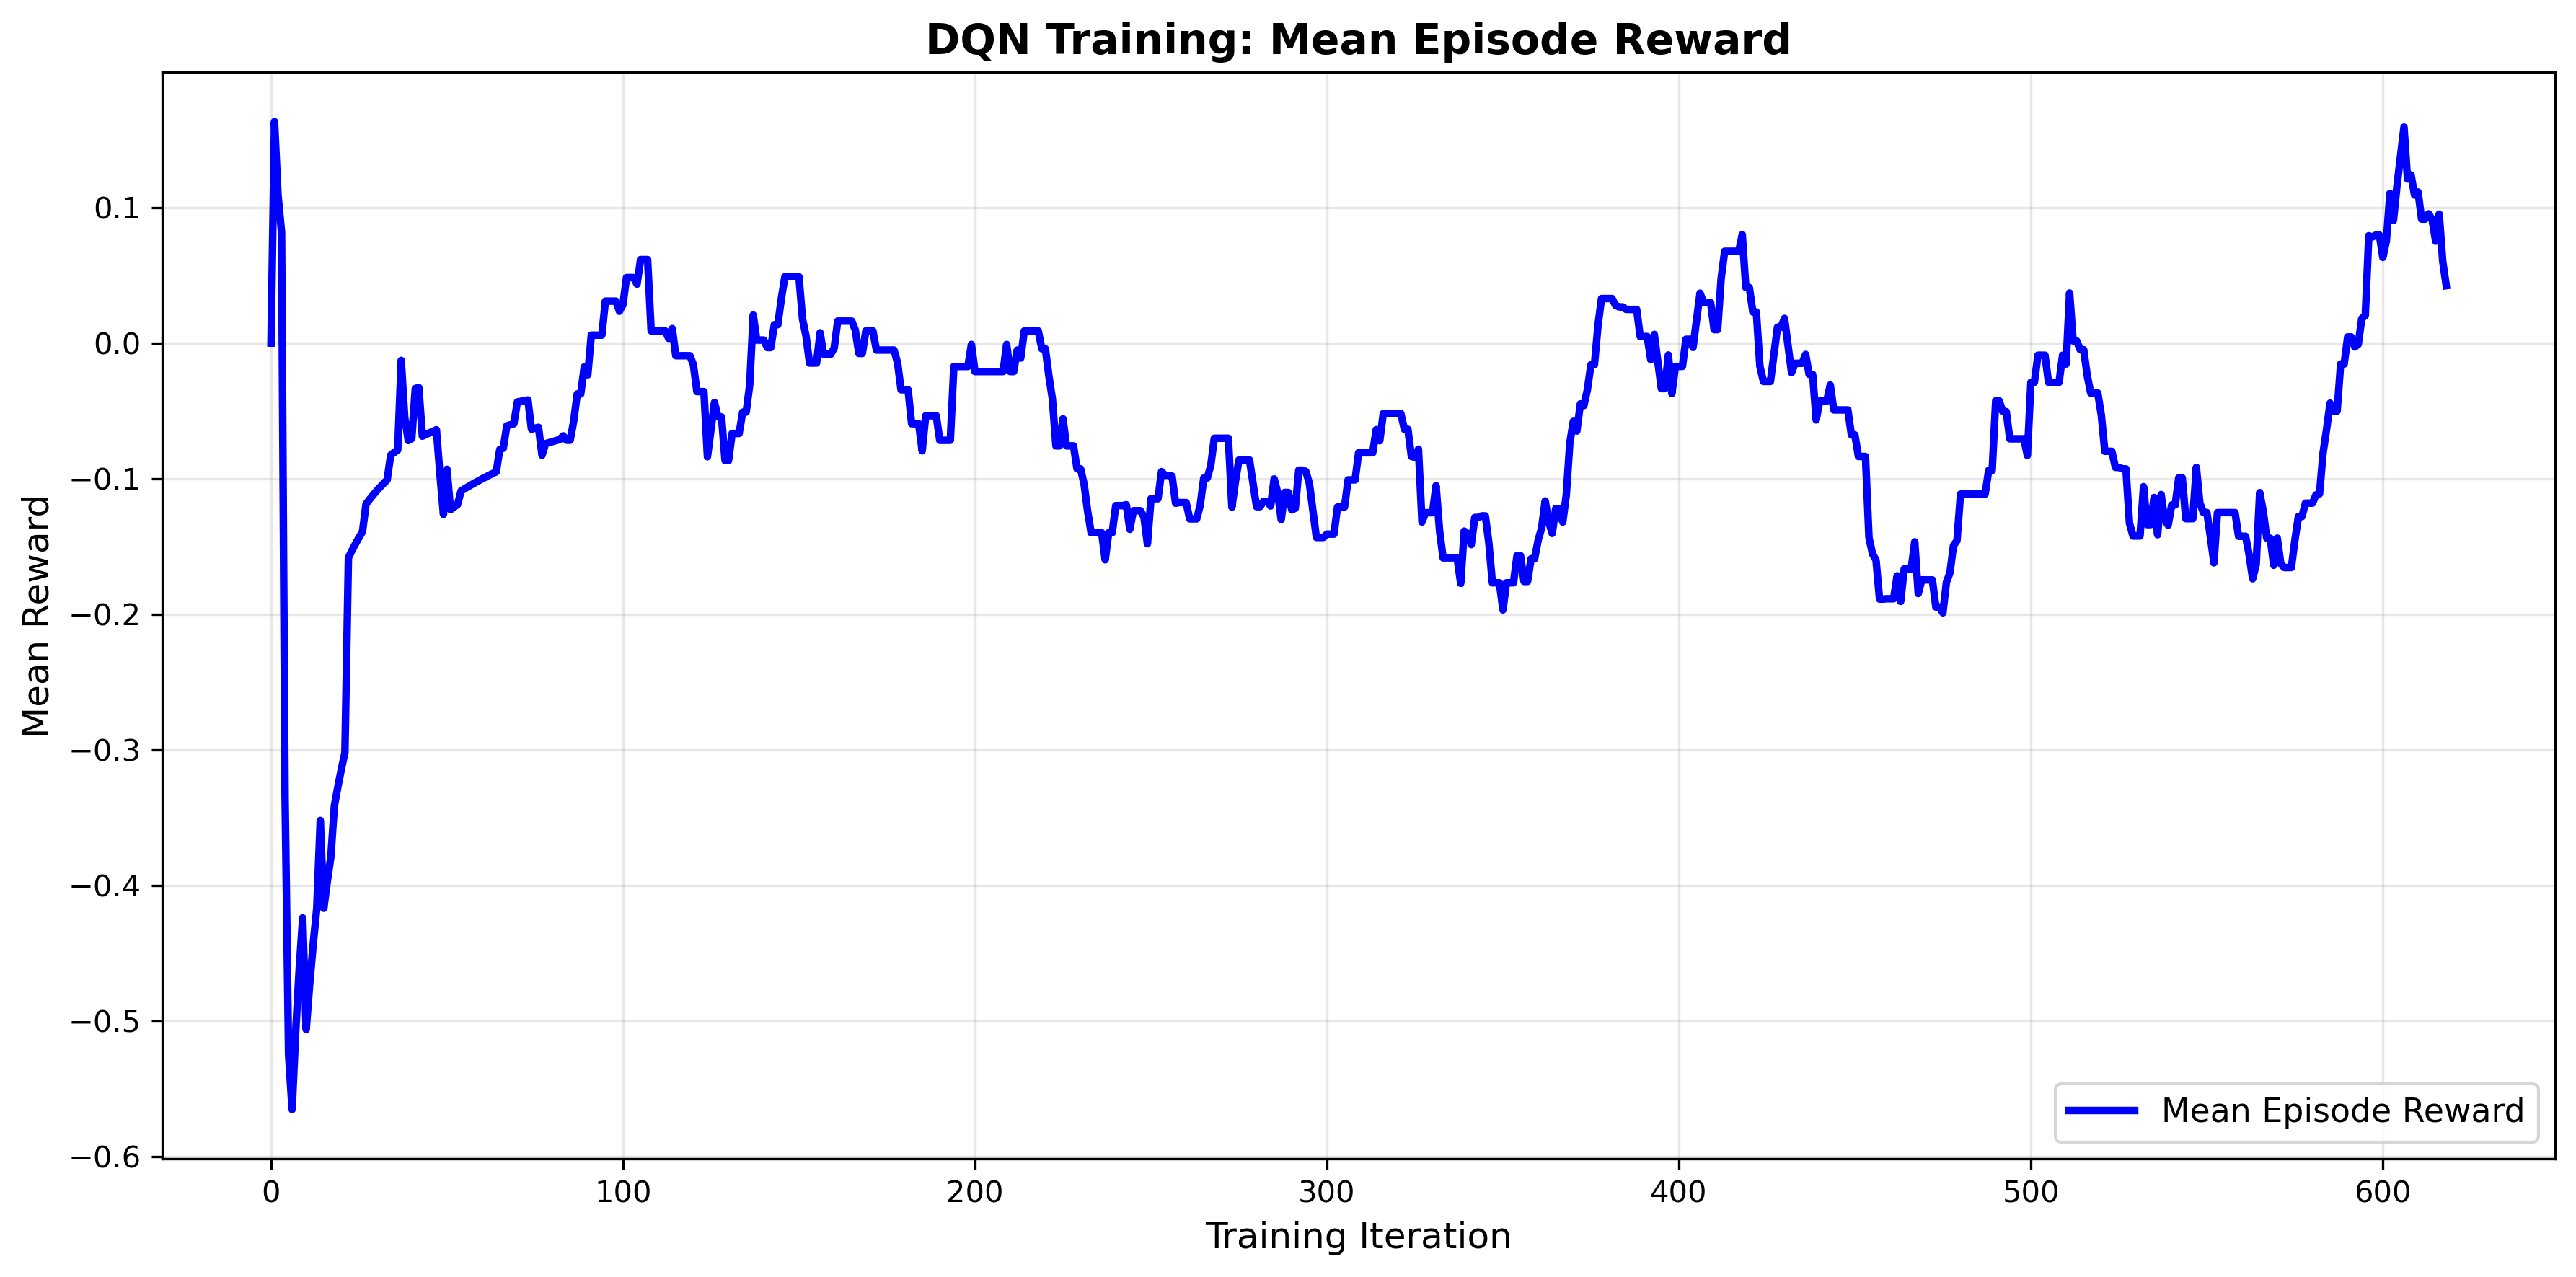
\includegraphics[width=0.9\textwidth]{mean_reward_curve.png}
\caption{Agent 2 (DQN with Custom Observation Wrapper): Mean episode reward across 100 training iterations. The curve demonstrates learning progression from initial exploration to refined value estimates.}
\label{fig:agent2_mean_reward}
\end{figure}

TODO: Add final checkpoint performance, win rate, average return, and comparison against Agent 1 or the same baselines.

	
%===============================================================================

\section{Conclusion}
\label{sec:conclusion}

\subsection{Agent 1 Conclusion}

TODO: Summarize whether PPO with curriculum learning and reward shaping improved learning and final Soccer Twos performance.

\subsection{Agent 2 Conclusion}

TODO: Summarize Agent 2's outcome and compare it with Agent 1.

	
%===============================================================================

\clearpage

%===============================================================================

% no \bibliographystyle is required, since the corl style is automatically used.
\bibliography{example}  % .bib

\end{document}
